% ----------------------------------------------------------------- %
%             The Speech Signal Processing Toolkit (SPTK)           %
%             developed by SPTK Working Group                       %
%             http://sp-tk.sourceforge.net/                         %
% ----------------------------------------------------------------- %
%                                                                   %
%  Copyright (c) 1984-2007  Tokyo Institute of Technology           %
%                           Interdisciplinary Graduate School of    %
%                           Science and Engineering                 %
%                                                                   %
%                1996-2017  Nagoya Institute of Technology          %
%                           Department of Computer Science          %
%                                                                   %
% All rights reserved.                                              %
%                                                                   %
% Redistribution and use in source and binary forms, with or        %
% without modification, are permitted provided that the following   %
% conditions are met:                                               %
%                                                                   %
% - Redistributions of source code must retain the above copyright  %
%   notice, this list of conditions and the following disclaimer.   %
% - Redistributions in binary form must reproduce the above         %
%   copyright notice, this list of conditions and the following     %
%   disclaimer in the documentation and/or other materials provided %
%   with the distribution.                                          %
% - Neither the name of the SPTK working group nor the names of its %
%   contributors may be used to endorse or promote products derived %
%   from this software without specific prior written permission.   %
%                                                                   %
% THIS SOFTWARE IS PROVIDED BY THE COPYRIGHT HOLDERS AND            %
% CONTRIBUTORS "AS IS" AND ANY EXPRESS OR IMPLIED WARRANTIES,       %
% INCLUDING, BUT NOT LIMITED TO, THE IMPLIED WARRANTIES OF          %
% MERCHANTABILITY AND FITNESS FOR A PARTICULAR PURPOSE ARE          %
% DISCLAIMED. IN NO EVENT SHALL THE COPYRIGHT OWNER OR CONTRIBUTORS %
% BE LIABLE FOR ANY DIRECT, INDIRECT, INCIDENTAL, SPECIAL,          %
% EXEMPLARY, OR CONSEQUENTIAL DAMAGES (INCLUDING, BUT NOT LIMITED   %
% TO, PROCUREMENT OF SUBSTITUTE GOODS OR SERVICES; LOSS OF USE,     %
% DATA, OR PROFITS; OR BUSINESS INTERRUPTION) HOWEVER CAUSED AND ON %
% ANY THEORY OF LIABILITY, WHETHER IN CONTRACT, STRICT LIABILITY,   %
% OR TORT (INCLUDING NEGLIGENCE OR OTHERWISE) ARISING IN ANY WAY    %
% OUT OF THE USE OF THIS SOFTWARE, EVEN IF ADVISED OF THE           %
% POSSIBILITY OF SUCH DAMAGE.                                       %
% ----------------------------------------------------------------- %
\hypertarget{dtw}{}
\name{dtw}{dynamic time warping}{dynamic time warping}
\begin{synopsis}
\item[dtw] [ --m $M$ ]  [ --l $L$ ]  [ --t $T$ ]  [ --r $R$ ]
           [ --n $N$ ]  [ --p $P$ ]
 \item [\ ~~~~~~~] [ --s $Scorefile$ ]  [ --v $OutVitfile$ ] [ --V $InVitfile$ ]
 {\em reffile} [ {\em infile} ]
\end{synopsis}

\begin{qsection}{DESCRIPTION}
 {\em dtw} carries out dynamic time warping (DTW) between the test data vectors from
 {\em infile} (or standard input) and the reference data vectors from {\em reffile},
 and sends the result to standard output.  The result is the concatenated sequence of
 the test and the reference data vectors along the Viterbi path.  If --s option is
 specified, the score calculated by dynamic time warping, that is, the distance
 between the test data and the reference data is output and sent to {\em Scorefile}.
 If --v option is specified, the concatenated frame number sequence along the Viterbi
 path is output and sent to {\em OutVitfile}.  On the other hand, if --V option is
 specified, the concatenated vector sequence of the test and reference data vectors
 is output based on the content of {\em InVitfile}, where the correspondence of the
 frame numbers between the test and reference data along the Viterbi path is written.
 The format of {\em InVitfile} is the same as {\em OutVitfile}.  The --V option can
 be used to improve the conversion accuracy of \hyperlink{vc}{vc} command.

 For example, suppose that the sequences of the test and the reference data vectors are
 \begin{align}
  \mathrm{test} :\;\; & \bx(1), \bx(2), \dots, \bx(T_x - 1), \bx(T_x), \notag \\
  \mathrm{reference}  :\;\; & \by(1), \by(2), \dots, \by(T_y - 1), \by(T_y), \notag
 \end{align}
 where $T_x$ and $T_y$ are the length of the sequence of the test and reference data
 vectors, respectively. After performing DTW, the following Viterbi sequences
 \begin{align}
  \mathrm{test} :\;\; & \bx(\phi_x(1)), \bx(\phi_x(2)), \dots, \bx(\phi_x(T - 1)),
  \bx(\phi_{x}(T)), \notag \\
  \mathrm{reference}  :\;\; & \by(\phi_y(1)), \by(\phi_y(2)), \dots,
  \by(\phi_y(T - 1)), \by(\phi_y(T)), \notag
 \end{align}
 can be obtained, where $\phi_x(\cdot)$ and $\phi_x(\cdot)$ are the function which
 maps the Viterbi frame number into the corresponding frame number of test/reference
 data, respectively.  Then, the following sequence
 \begin{align}
  \bx(\phi_x(1)), \by(\phi_y(1)),
  \bx(\phi_x(2)), \by(\phi_y(2)),
  \dots, \bx(\phi_{x}(T)), \by(\phi_y(T)) \notag
 \end{align}
 is sent to the standard output.
 If --v option is specified, the following sequence
 \begin{align}
  \phi_x(1), \phi_y(1),
  \phi_x(2), \phi_y(2),
  \dots, \phi_{x}(T), \phi_y(T) \notag
 \end{align}
 is sent to the {\em OutVitfile}.
 On the other hand, if --V option is specified, according to the following sequence
 written in {\em InVitfile}
 \begin{align}
  \phi_x(1), \phi_y(1),
  \phi_x(2), \phi_y(2),
  \dots, \phi_{x}(T), \phi_y(T), \notag
 \end{align}
 the following concatenated vector sequence
 \begin{align}
  \bx(\phi_x(1)), \by(\phi_y(1)),
  \bx(\phi_x(2)), \by(\phi_y(2)),
  \dots, \bx(\phi_{x}(T)), \by(\phi_y(T)) \notag
 \end{align}
 can be obtained and sent to the standard output.

 Both input and output files are in float format. However,
 {\em InVitfile} and {\em OutVitfile} which contains the Viterbi frame number
 sequence is in int format.
\end{qsection}
\begin{options}
 \argm{m}{M}{order of vector}{0}
 \argm{l}{L}{dimention of vector}{M+1}
 \argm{t}{T}{number of test vectors}{N/A}
 \argm{r}{R}{number of reference vectors}{N/A}
 \argm{n}{N}{type of norm used for calculation of local cost\\
 \begin{tabular}{ll} \\[-1ex]
  $N=1$ & ~~~$L_{1}$-norm\\
  $N=2$ & ~~~$L_{2}$-norm\\
 \end{tabular}\\\hspace*{\fill}}{2}
 \argm{p}{P}{local path constraint\\
 candidates of constraint are shown in figure \ref{fig:dtw_cand}.}{5}
 \argm{s}{Scorefile}{output score of the dynamic time warping
 to ${Scorefile}$. }{FALSE}
 \argm{v}{OutVitfile}{output frame number sequence along the Viterbi
 path to ${OutVitfile}$.}{FALSE}
 \argm{V}{InVitfile}{concatenate test and reference vectors along the Viterbi
 path information written in ${InVitfile}$.}{FALSE}
\end{options}

\begin{qsection}{EXAMPLE}
 In the example below, a dynamic time warping between the scalar
 sequence from {\em data.test} and
 the sequence from {\em data.ref} is carried out and
 the concatenated sequence are written to {\em data.out}.
\begin{quote}
 \verb!dtw -l 1 data.ref < data.test > data.out!
\end{quote}
\end{qsection}

\begin{figure}[htbp]
 \begin{center}
  \begin{tabular}{cccc} \\[-1ex]
   &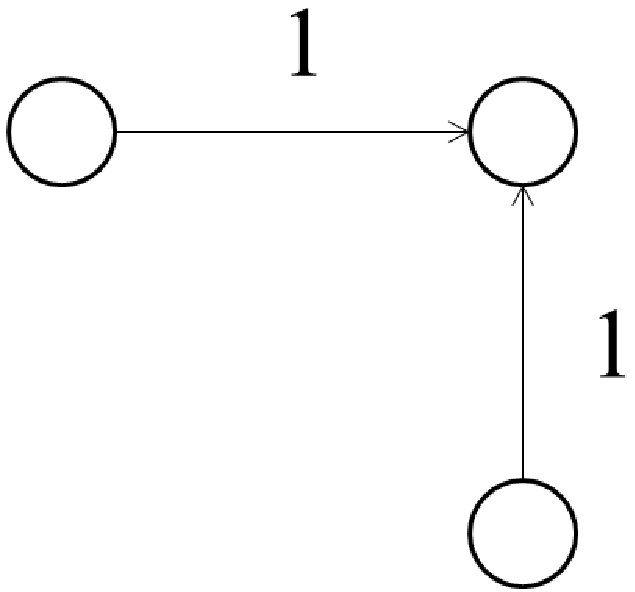
\includegraphics[height=2cm]{fig/path1.pdf}
   &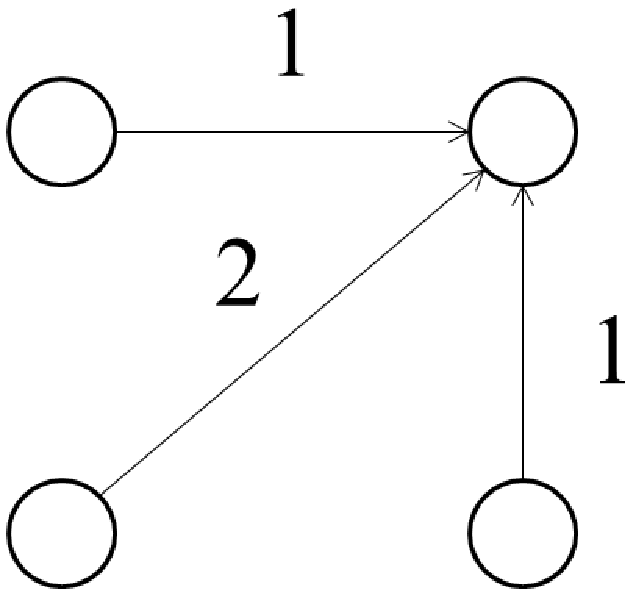
\includegraphics[height=2cm]{fig/path2.pdf}
   &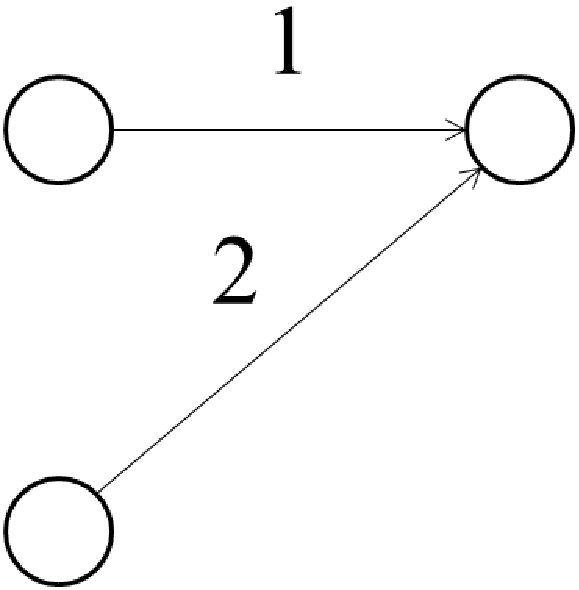
\includegraphics[height=2cm]{fig/path3.pdf}\\
   &$P=1$&$P=2$&$P=3$\\
   &&&\\
   &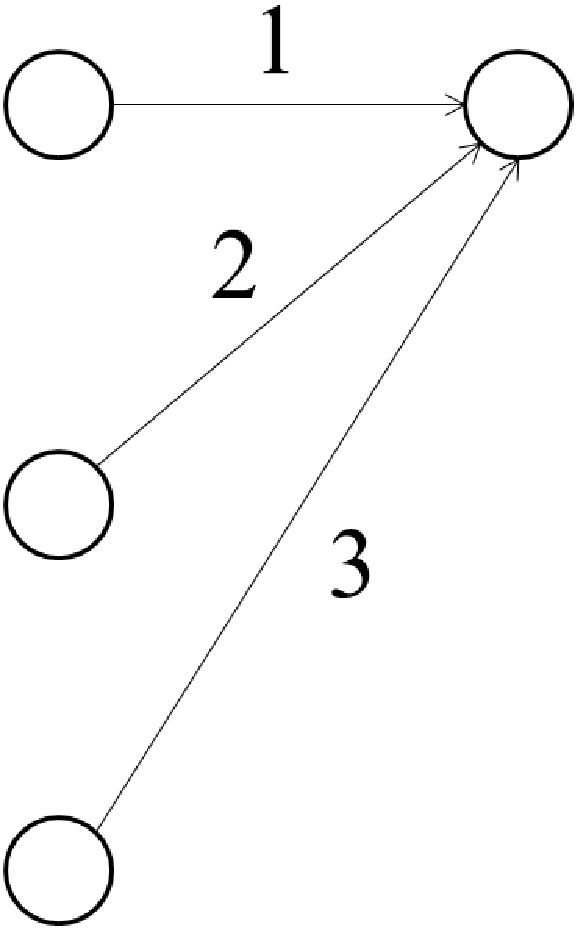
\includegraphics[height=3cm]{fig/path4.pdf}
       &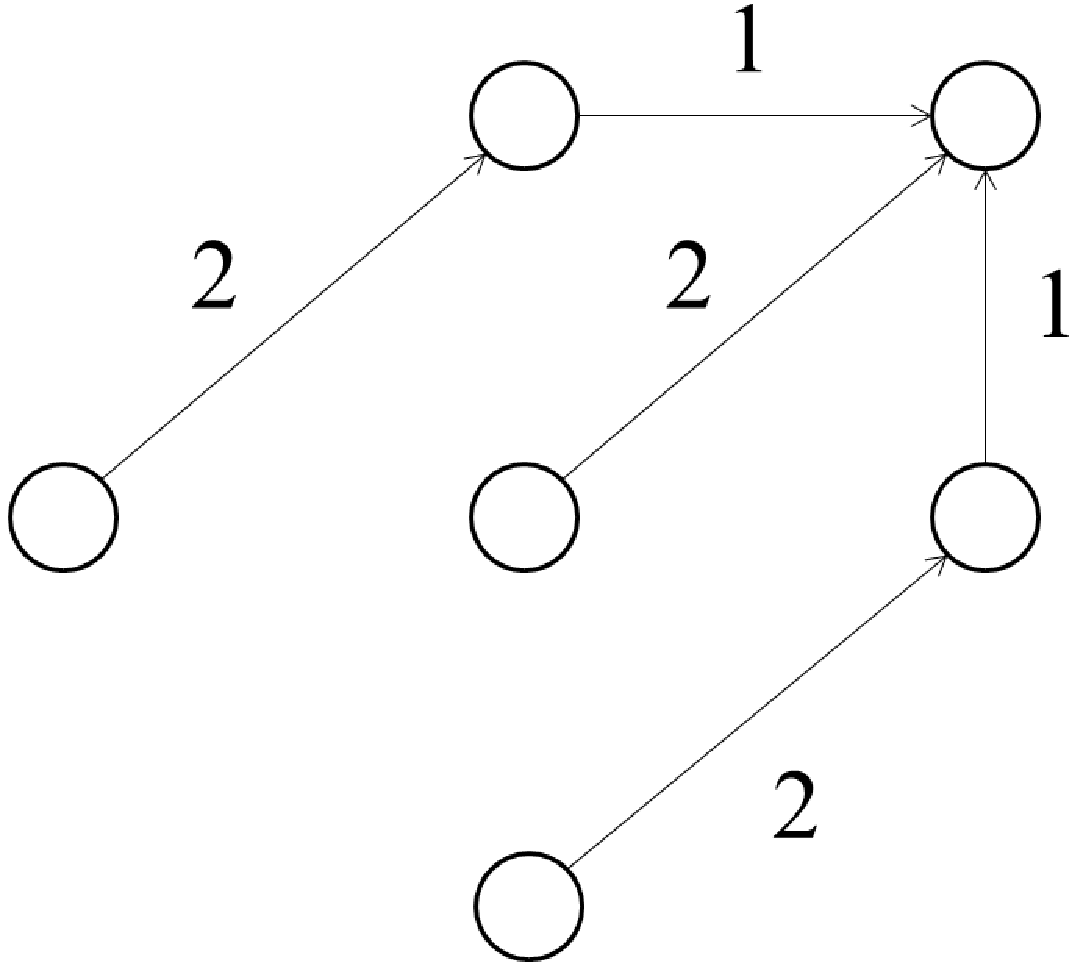
\includegraphics[height=3cm]{fig/path5.pdf}
   &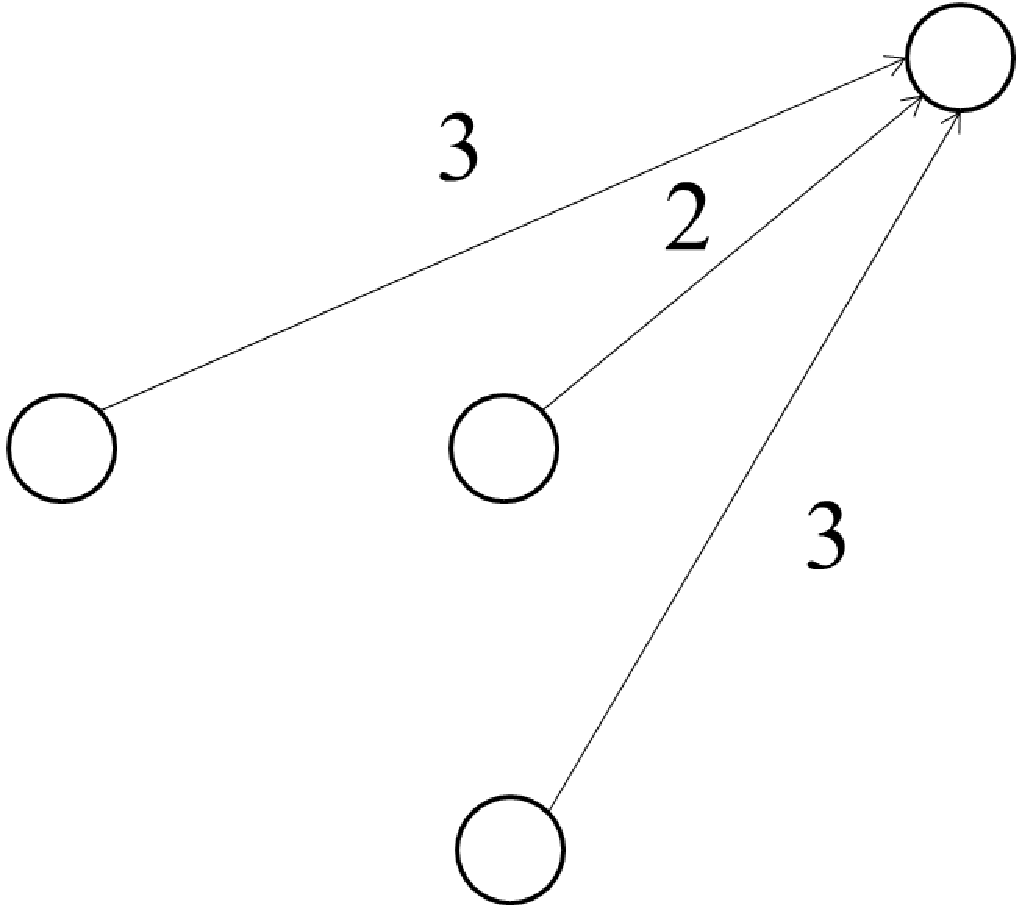
\includegraphics[height=3cm]{fig/path6.pdf}\\
   &$P=4$&$P=5$&$P=6$\\
   &&&\\
   &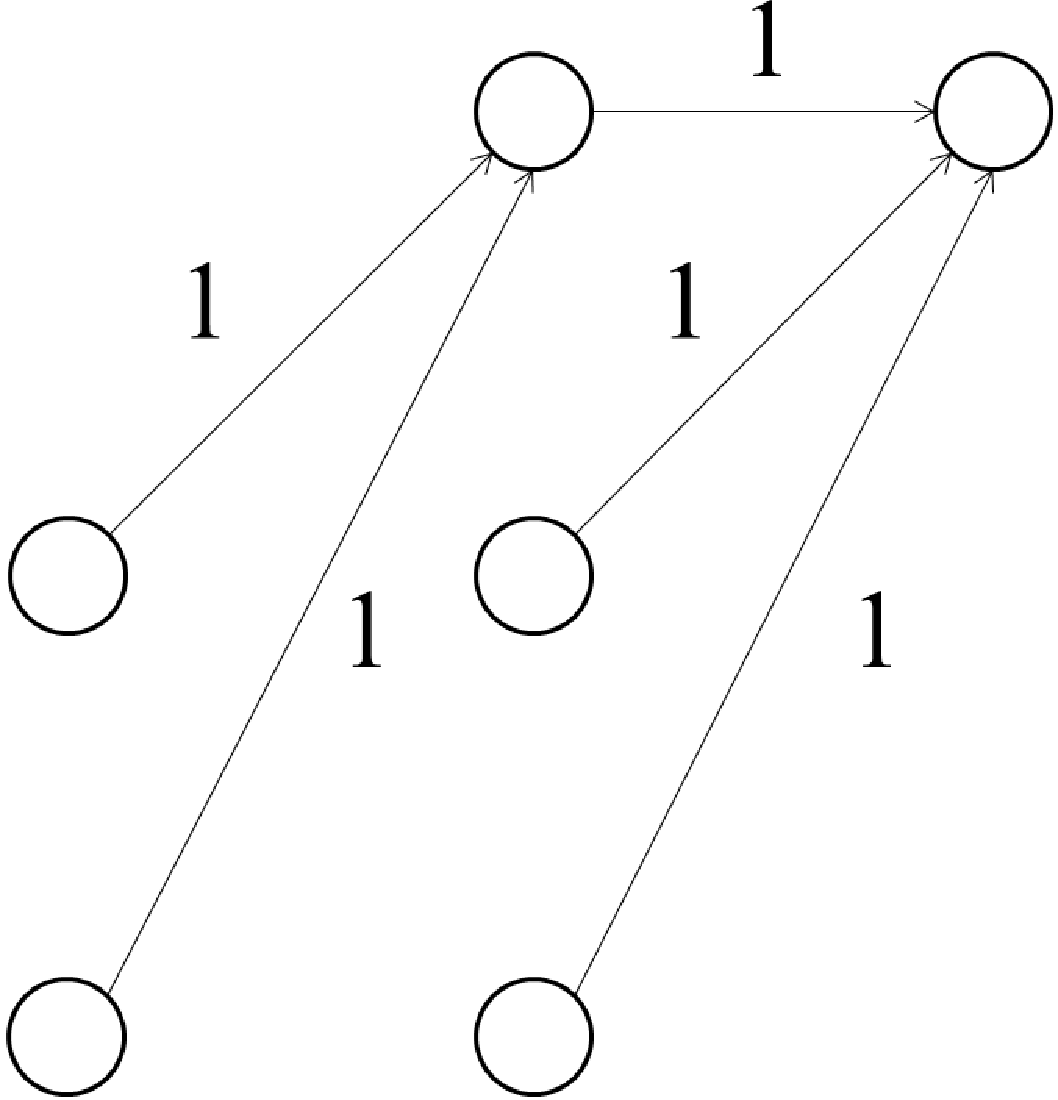
\includegraphics[height=3cm]{fig/path7.pdf}
       &&\\
   &$P=7$&&\\
  \end{tabular}
 \end{center}
 \caption{candidates of local path constraint}
 \label{fig:dtw_cand}
\end{figure}

\begin{qsection}{SEE ALSO}
\hyperlink{vc}{vc}
\end{qsection}
